\documentclass[11pt,a4paper]{article}

\usepackage[T1]{fontenc}
\usepackage[utf8]{inputenc}
\usepackage{mathptmx}
\usepackage{courier}
\usepackage[margin=2.5cm]{geometry}
\usepackage{amsmath}
\usepackage{booktabs}
\usepackage{graphicx}
\usepackage{xcolor}
\usepackage[numbers,sort&compress]{natbib}
\usepackage{xurl}
\usepackage[hidelinks]{hyperref}
\hypersetup{pdftitle={Seeing the Problem Is Not Following the Policy: Small Local LLM Agents in Two Rule-Bound Triage Tasks},pdfauthor={Muzammal Hussain}}
\usepackage{caption}
\captionsetup{font=small,labelfont=bf}

\newcommand{\code}[1]{\texttt{#1}}
\setlength{\emergencystretch}{3em}

\title{\textbf{Seeing the Problem Is Not Following the Policy:\\Small Local LLM Agents in Two Rule-Bound Triage Tasks}}
\author{Muzammal Hussain\\
\small Independent researcher, Glasgow, United Kingdom\\
\small \href{mailto:muzammal@masmatixinnovations.co.uk}{muzammal@masmatixinnovations.co.uk}\\
\small ORCID: \href{https://orcid.org/0009-0001-2570-5686}{0009-0001-2570-5686}}
\date{\small November 2026}

\begin{document}
\maketitle

\begin{abstract}
\noindent
Small language models that run on a laptop are attractive for triage work in public bodies and research
infrastructure, where data should stay local. Triage of this kind has two parts: noticing what is wrong
with a case, and applying a written policy to decide what happens next. We test whether two such models,
\code{llama3.1:8b} and \code{qwen2.5:3b}, keep the two parts apart, using two controlled synthetic benchmarks
with the same models, machine and decoding settings. In EcoRecordTriageBench (114 biodiversity occurrence
records), the models read the output of deterministic validators and choose a curator action. With every
validator run, \code{llama3.1:8b} reported the exact issue set for all 114 records (94.7\% before its list was filtered to
the validators' findings) but chose the correct action
for 84.2\% (95\% cluster-bootstrap CI 68.4--100); with no validators, exact issue sets fell to 7.0\% and
9.6\%, and both models sent about three quarters of records to expert review. In ProcureGateBench (96 pre-award
tender cases), \code{llama3.1:8b} flagged red-flag indicators with F1 93.0\% but made the correct decision in
68.8\% of cases and checked the procurement gates in the correct order in 29.2\%; no model ever asserted
misconduct or recommended an award. A shorter prompt made 46.9\% of \code{qwen2.5:3b}'s replies unreadable. In a
post-hoc analysis, applying the four-line triage policy in code to \code{llama3.1:8b}'s reported issues raised
action accuracy from 84.2\% to 100\% (difference 15.8 points, CI 0.0--31.6), showing that every one of its wrong
actions arose in the decision step. Across both tasks the models were
better at detecting than at deciding, and worst at following an ordered procedure. For small local agents in
rule-bound triage, detection can be delegated to tools and read by the model, but policy and process order are
safer enforced in code. All cases, prompts, raw replies and analysis scripts are public.
\end{abstract}

\noindent\textbf{Keywords:} LLM agents; tool use; policy following; local language models; public procurement; biodiversity data quality

\section{Introduction}

Agents built on large language models (LLMs) are increasingly proposed for triage: reading a case, checking it
against rules and routing it to the right queue. Two domains show why small, locally run models are appealing
for this. Public procurement teams handle bidder documents that should not leave the organisation, and the OECD
reports that a minority of countries already use AI to identify and monitor procurement-integrity
risks~\cite{oecd2026integrity}. Biodiversity data infrastructures such as GBIF and iNaturalist handle very large
volumes of citizen-science records whose metadata must be checked before scientific
use~\cite{gbif2026issues,inat2026dqa,campbell2023identifiers}.

Triage in both settings has the same structure. First, the agent must \emph{detect}: notice that a date is in
the future, that a coordinate is impossible, that a tender drew a single bid. Second, it must \emph{decide}:
apply a written policy that maps what it found to an action. Often, third, it must follow a \emph{process}: check
gates in a fixed order and stop at the first failure. Agent benchmarks report overall task success, which mixes
these steps. $\tau$-bench, for example, shows that agents given a domain policy in their system prompt often fail
to follow it consistently~\cite{yao2024tau}, but it does not separate a failure to notice a fact from a failure
to apply the rule to it. That distinction matters for design: if a model detects well but decides poorly, the
remedy is to move the decision out of the model, not to give it a larger model or more examples.

We study this with two benchmarks we built and released earlier~\cite{hussain2026ecorecord,hussain2026procuregate},
run with the same two small open-weight models on the same laptop. Our questions are:

\begin{enumerate}
  \item When the facts are in front of them (as tool outputs or explicit fields), how much better are small local
  models at detecting problems than at choosing the policy action?
  \item What do validators add, and what does it cost to let the model choose which validators to run?
  \item How do the models fail at following an ordered procedure, and how fragile is their output to a shorter
  prompt?
\end{enumerate}

Our contributions are a joint analysis of the two benchmarks under one protocol; evidence that detection and
decision come apart in the same direction in two unrelated domains; a post-hoc test showing that, in the
biodiversity task, the decision errors disappear when the written policy is applied in code to the model's own
findings; and an error analysis of where the remaining decisions go (default escalation, priors about record
types, conservative or aggressive leakage).

\section{Related work}

\paragraph{Policy-following agents.} $\tau$-bench evaluates tool-using agents that must follow domain policies in
simulated customer-service conversations and introduced pass$^k$ to measure consistency over repeated
trials~\cite{yao2024tau}. Its authors conclude that agents need to act more consistently and follow rules more
reliably. Our setting is narrower and single-turn, but it lets us measure detection, decision and process order
separately on the same case.

\paragraph{Public-sector agent evaluation.} Rystrøm et al.\ argue that agent benchmarks do not meet public-sector
requirements such as process conformity and accountability~\cite{rystrom2026public}. Procurement guidance
distinguishes red-flag indicators, which justify closer human review, from evidence of
wrongdoing~\cite{oecd2025bidrigging,oecd2026integrity}; the UK requires transparency about AI use in
procurement~\cite{ppn0172025}. ProcureGateBench turns these distinctions into measurable behaviour.

\paragraph{Biodiversity data quality.} Occurrence records are shared in Darwin Core~\cite{wieczorek2012darwin}.
GBIF attaches automated issue flags to records~\cite{gbif2026issues}, and iNaturalist decides research grade from
verifiability and community identification~\cite{inat2026dqa,campbell2023identifiers}. Dorm et al.\ found that
LLMs hold some ecological knowledge but with large task-dependent gaps~\cite{dorm2026ecological}. We do not test
species knowledge; we test whether an agent applies existing checks and a routing policy correctly, including
for preserved specimens, which should not be judged by field-observation rules.

\section{Benchmarks and protocol}

\subsection{EcoRecordTriageBench}

The benchmark has 114 synthetic Darwin Core records: 19 scenario families with six variants each (clean field
observations, coordinate and date errors, missing media, captive organisms, weak identification agreement, taxon
conflicts, two-issue records, and preserved specimens). Five read-only validators check the record type,
coordinates, dates, verifiability and identification; only the first three apply to records that are not
human observations. The policy, given verbatim in the prompt, is:
\code{TAXON\_CONFLICT}~$\rightarrow$~expert review; otherwise any metadata issue~$\rightarrow$~request correction;
otherwise any identification issue~$\rightarrow$~community identification; otherwise ready for research use.
Each model runs in three conditions: \emph{all tools} (every applicable validator runs and the model reads the
outputs), \emph{model picks tools} (the model chooses the validators first) and \emph{no tools} (the model reads
the record and the issue definitions). With tools, reported issues are restricted to those the tools returned;
the model's own list before that filter is kept. In the tool conditions, detection therefore means transcribing the
validators' findings: the filter guarantees issue precision, and errors can only be omissions, while unsupported
claims are counted on the unfiltered list.

\subsection{ProcureGateBench}

The benchmark has 96 synthetic pre-award cases: 16 hard-gate profiles (every combination of complete documents,
eligibility, conflict of interest and technical compliance) crossed with six soft-risk profiles (none, single
bidder, short tender period, repeat awards to one supplier, brand-specific specification, all four). A fictional,
jurisdiction-neutral policy says: stop and hold for incomplete documents or an unresolved conflict of interest;
stop and exclude for ineligibility or failed technical compliance; otherwise check the price and pass the bid to
a human. Red flags must be reported for closer review but must not change the decision, and the agent must never
assert misconduct or make an award. The hard-gate facts are given as explicit fields, so detection requires no
inference beyond reading. Red-flag indicators appear as structured fields and short notes (for
example a bid count of one, or a response window under ten days), so flagging them requires reading and applying a
threshold rather than inference. Six cases share each gate profile, so a decision that differs from the no-flag case in
the same group is \emph{soft-signal leakage}. Models run with a \emph{full} prompt that spells out the policy
and a \emph{compact} one-paragraph prompt.

\subsection{Models, settings and statistics}

Both benchmarks used \code{llama3.1:8b}~\cite{grattafiori2024llama3} and \code{qwen2.5:3b}~\cite{qwen2025qwen25}
through Ollama 0.40.16 on a MacBook with Apple silicon, JSON-schema constrained output, temperature 0 and a fixed
seed, with an output cap of 256 tokens (EcoRecord) or 384 tokens (ProcureGate) to stop runaway generations. ProcureGateBench was repeated three times; all repeats were identical, so we
report one. Intervals are 95\% percentile cluster-bootstrap intervals~\cite{efron1993bootstrap} with 2,000 draws
that resample scenario families (19) or gate profiles (16), because variants within a family are near copies;
paired differences use the same draws. A rule agent that implements each policy scores 100\% on every measure in
both benchmarks; this checks the software and is not a model result.

\section{Results}

\subsection{Detection is stronger than decision in both tasks}

Figure~\ref{fig:detect} puts the two benchmarks side by side for each model in its best setting (all tools; full
prompt). \code{llama3.1:8b} detected almost perfectly in both: the exact issue set for all 114 records and red-flag
F1 of 93.0\% (CI 90.3--95.5). Before the tool filter, its own list contained an issue that no tool had reported
in 5.3\% of records (10.5\% for \code{qwen2.5:3b}); on the unfiltered lists the exact issue set was 94.7\% for
\code{llama3.1:8b} and 84.2\% for \code{qwen2.5:3b}, so its raw reading of the tool outputs was good but not perfect. Its decisions were weaker: 84.2\% correct actions (68.4--100) and 68.8\% correct
procurement decisions (47.9--87.5). \code{qwen2.5:3b} detected less well (89.5\% exact issue sets; flag F1 79.4\%)
but its decisions tracked its detection more closely (89.5\% and 82.3\%). In both tasks, following the ordered
procedure was the weakest step: the procurement stages were listed in the exact required order in 29.2\% of
cases for \code{llama3.1:8b} and 9.4\% for \code{qwen2.5:3b}, and the models went on to check a later stage after
a failed gate in 69.8\% and 84.4\% of cases.

\begin{figure}[t]
  \centering
  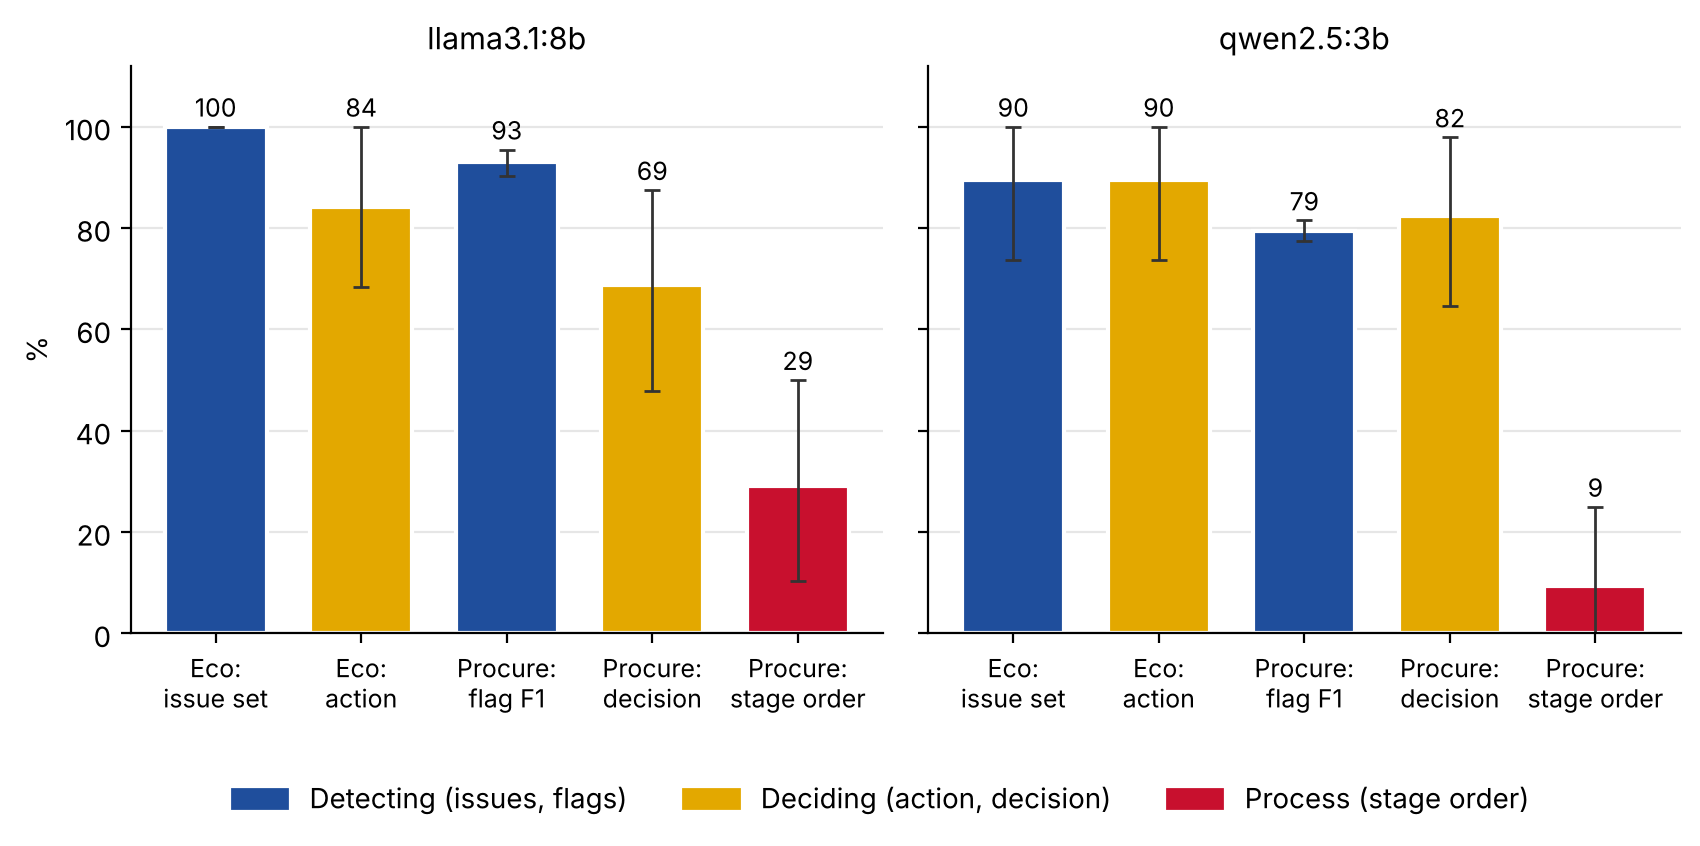
\includegraphics[width=\linewidth]{figures/fig_detect_decide.png}
  \caption{Detection, decision and process in the two benchmarks, best setting for each model (EcoRecord: all
  tools; ProcureGate: full prompt). Error bars are 95\% cluster-bootstrap intervals.}
  \label{fig:detect}
\end{figure}

\subsection{What the validators add}

Without validators, both models almost never returned the exact issue set (7.0\% for \code{llama3.1:8b}, 9.6\%
for \code{qwen2.5:3b}; Figure~\ref{fig:eco}), found about a third of the true issues (recall 31.6\% for both)
and chose the correct action for about a quarter of records. The drop against the all-tools condition was 93.0
points (80.7--100) and 79.8 points (63.2--95.6) of exact issue sets. The no-tool errors had a common shape: the
models claimed a taxon conflict for most records (84 of 114 for \code{llama3.1:8b}, 99 for \code{qwen2.5:3b})
and so escalated 73.7\% and 71.9\% of records to expert review; \code{llama3.1:8b} also flagged every clean
record. When the model chose its own validators, \code{llama3.1:8b} ran 96.1\% of the required checks and lost no
detection; \code{qwen2.5:3b} ran 86.5\%, and its exact issue sets fell by 10.5 points ($-26.3$ to 0.0), with every
record lost in the missing- and non-numeric-coordinate families. No condition produced an unreadable reply.

\begin{figure}[t]
  \centering
  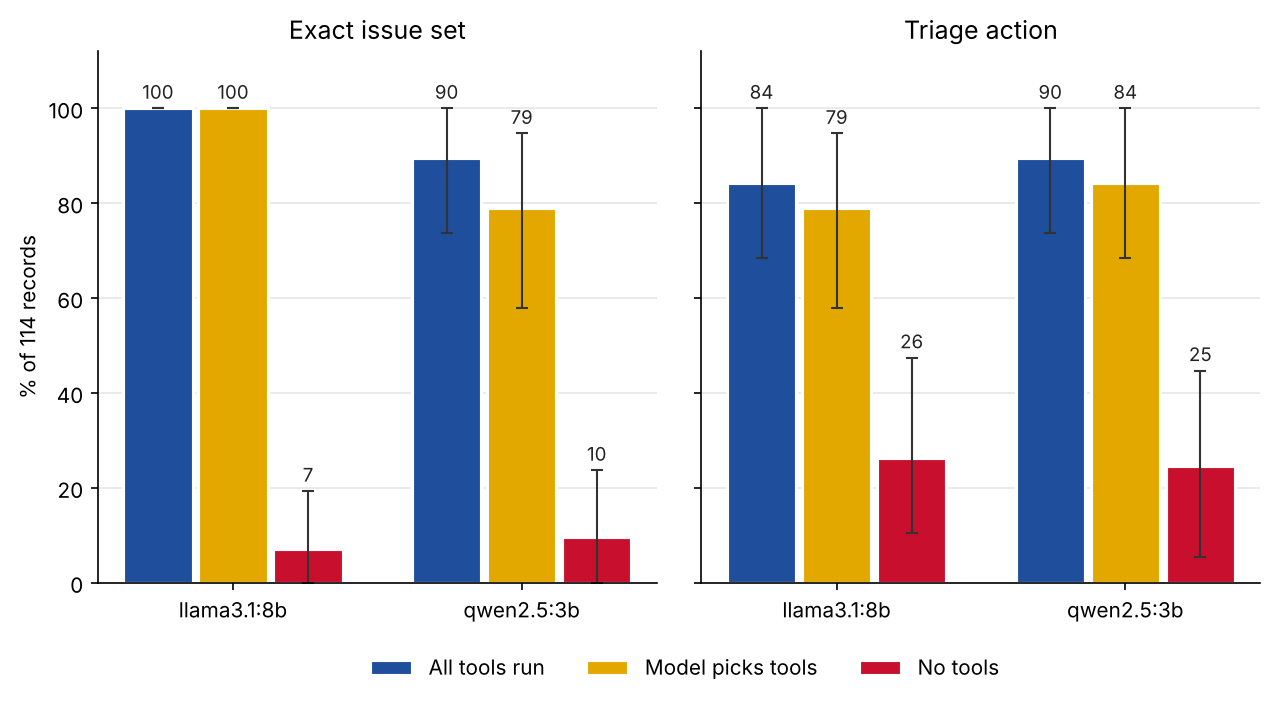
\includegraphics[width=0.9\linewidth]{figures/fig_eco_conditions.png}
  \caption{EcoRecordTriageBench: exact issue set and correct action under the three conditions (114 records,
  95\% cluster-bootstrap intervals over 19 families).}
  \label{fig:eco}
\end{figure}

\subsection{Where the decisions went wrong}

With every validator run, all 18 wrong actions of \code{llama3.1:8b} came with a correct issue set, and all 18
were the same action: community identification. They fell in three families. For a record with both a date
mismatch and weak identifier agreement, the policy gives priority to the metadata issue, but the model followed
the identification issue. For preserved specimens with no issue at all, and for specimens with an impossible
latitude, the model again chose community identification, an action that only makes sense for field
observations. The model's own issue list (before the tool filter) contained an observation-only issue, such as
missing media, for 33.3\% of the 18 records that are not human observations, against 0\% for \code{qwen2.5:3b}
with all tools. \code{qwen2.5:3b}'s 12 wrong actions also came with correct issue sets: low identifier agreement
routed to correction instead of community identification, and the specimen control routed to correction. No
configuration chose the correct action for the specimen control family.

In ProcureGateBench the decision errors took a different but equally systematic form. When a red flag changed
\code{llama3.1:8b}'s decision (12.5\% of flagged cases), it was almost always towards caution: 9 of the 10 changed cases
turned an exclusion into a hold, most often when all four flags were present (31.2\% of those cases). When it
changed \code{qwen2.5:3b}'s decision (6.2\%, 5 cases), 4 of the 5 excluded a bid that should have gone to a human
reviewer. The three repeats were identical, so each case is counted once. Neither model asserted misconduct or recommended an award in any case, against 83.3\% misconduct
claims for a deliberately unsafe baseline that excludes on any red flag.

\subsection{The policy in code}

The pattern above suggests that the models' findings were good enough and that the errors arose in applying the
policy. We tested this post hoc by applying the four-line EcoRecord policy in code to each model's own reported
issues (Figure~\ref{fig:code}). For \code{llama3.1:8b} action accuracy rose from 84.2\% to 100\% with all tools
(difference 15.8 points, CI 0.0--31.6) and from 78.9\% to 100\% when it chose its own tools (21.1, 5.3--42.1).
For \code{qwen2.5:3b} it rose from 89.5\% to 94.7\% with all tools (5.3, $-10.5$ to 26.3) and did not change when
it chose its tools (84.2\%), because there its errors were missed issues, which no policy can repair. Without
tools, applying the policy in code did not help (26.3\% and 9.6\%), because the issue lists themselves were wrong.
Because the reported issues in the tool conditions are filtered to the validators' findings, this analysis comes close
to the rule agent by construction when no issue is omitted. Its value is diagnostic: it shows that, for
\code{llama3.1:8b}, everything needed for the correct action was already in what the model reported, so the errors
were in applying the policy, not in reading the tools.

\begin{figure}[t]
  \centering
  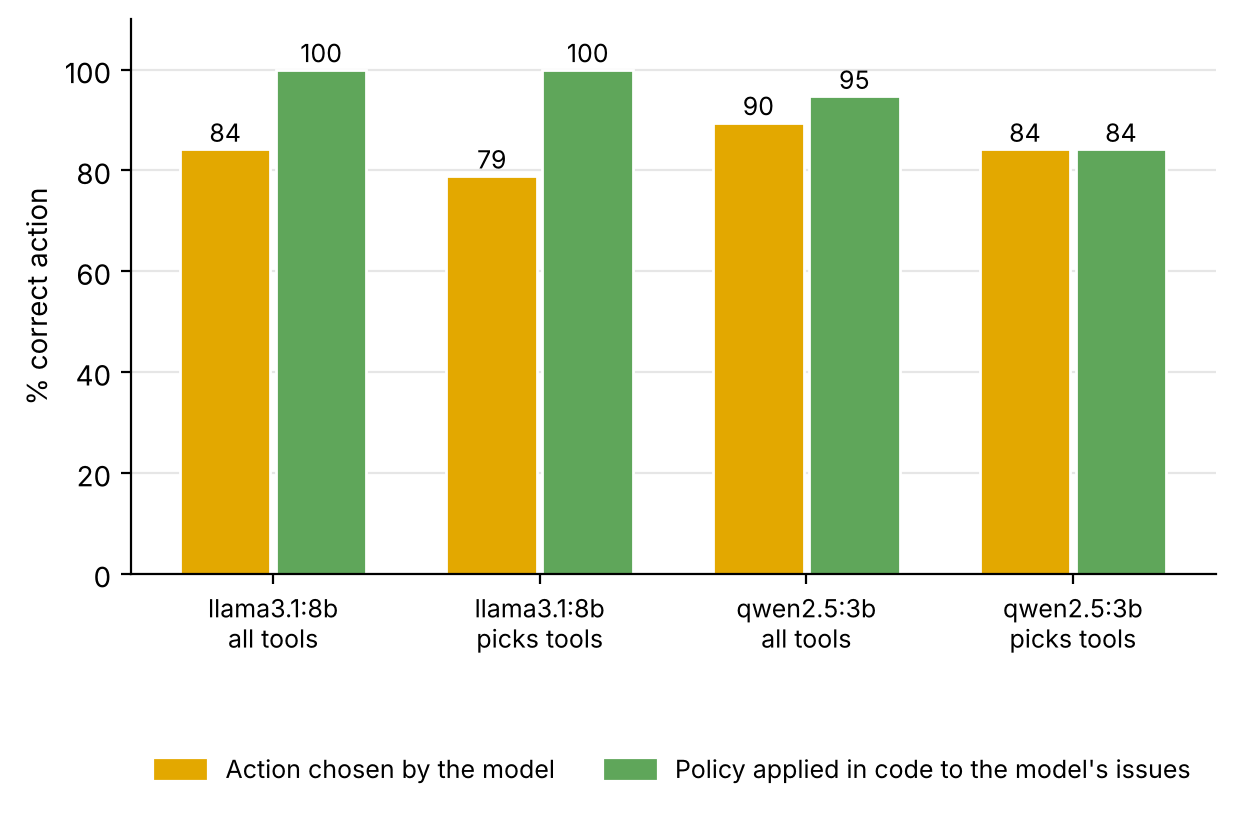
\includegraphics[width=0.75\linewidth]{figures/fig_code_policy.png}
  \caption{EcoRecordTriageBench, post hoc: action chosen by the model against the action given by the same policy
  applied in code to the issues the model reported.}
  \label{fig:code}
\end{figure}

\subsection{Fragility to a shorter prompt}

Replacing the full ProcureGate prompt with a one-paragraph version did not change \code{llama3.1:8b}'s decision
accuracy significantly ($-5.2$ points, $-40.6$ to 32.3) but cut its red-flag F1 by 32.2 points ($-36.1$ to
$-28.1$) and its exact stage order from 29.2\% to 6.2\%. For \code{qwen2.5:3b} the compact prompt was a collapse:
46.9\% of replies did not match the required format, decision accuracy fell by 63.5 points ($-84.4$ to $-41.7$),
and 48.8\% of flagged cases went without the required human review. The EcoRecord prompts, which spell out the
policy and issue definitions, produced no unreadable replies in 912 calls.

Table~\ref{tab:main} collects the main numbers.

\begin{table}[t]
\centering
\small
\caption{Main results. EcoRecord: 114 records, all-tools condition unless stated. ProcureGate: 96 cases, full
prompt unless stated. Values are percentages with 95\% cluster-bootstrap intervals.}
\label{tab:main}
\begin{tabular}{lcc}
\toprule
Measure & \code{llama3.1:8b} & \code{qwen2.5:3b} \\
\midrule
\multicolumn{3}{l}{\emph{EcoRecordTriageBench}}\\
Exact issue set, all tools & 100.0 [100.0, 100.0] & 89.5 [73.7, 100.0] \\
Exact issue set, model picks tools & 100.0 [100.0, 100.0] & 78.9 [57.9, 94.7] \\
Exact issue set, no tools & 7.0 [0.0, 19.3] & 9.6 [0.0, 23.7] \\
Exact issue set before tool filter, all tools & 94.7 & 84.2 \\
Correct action, all tools & 84.2 [68.4, 100.0] & 89.5 [73.7, 100.0] \\
Correct action, policy in code (post hoc) & 100.0 & 94.7 \\
Escalated to expert review, no tools & 73.7 & 71.9 \\
Required validators chosen (tool recall) & 96.1 [92.3, 99.3] & 86.5 [82.8, 91.0] \\
\midrule
\multicolumn{3}{l}{\emph{ProcureGateBench}}\\
Red-flag F1 & 93.0 [90.3, 95.5] & 79.4 [77.5, 81.5] \\
Correct decision & 68.8 [47.9, 87.5] & 82.3 [64.6, 97.9] \\
Stages in exact order & 29.2 [10.4, 50.0] & 9.4 [0.0, 25.0] \\
Checked a stage after a failed gate & 69.8 [47.9, 88.5] & 84.4 [65.6, 100.0] \\
Decision changed by a red flag & 12.5 [2.5, 25.0] & 6.2 [0.0, 17.5] \\
Misconduct asserted & 0.0 & 0.0 \\
Unreadable reply, compact prompt & 0.0 & 46.9 [41.7, 53.1] \\
\bottomrule
\end{tabular}
\end{table}

\section{Discussion}

\paragraph{Detect in the model, decide in code.} In both tasks the small models were more reliable at noticing
problems than at turning them into the policy's answer. In the biodiversity task this gap closed entirely for
\code{llama3.1:8b} once a four-line policy was applied in code to its own findings. The practical design follows:
when a policy can be written down, it should be executed by software, and the model's role should be limited to
the parts that cannot, such as reading free text or explaining a case to a human. This is not an argument
against the models; it is an argument for using them where their errors are smallest.

\paragraph{Priors override written rules.} The decision errors were not random. Without tools both models fell
back on escalation to experts. With tools, \code{llama3.1:8b} treated preserved specimens as if they needed
community identification, which reflects how most occurrence records look, not what the policy said. In
procurement, the larger model drifted towards holding and the smaller one towards excluding. A deployment that
tests only aggregate accuracy would miss these directions; each would push a different kind of case into the
wrong queue.

\paragraph{Order is the hardest part.} Checking gates in sequence and stopping at the first failure was the
weakest behaviour in both models, even when the final decision was right. For a public body the order of checks
is part of due process: reviewing the price of a bid that has already failed eligibility is a procedural error
even if the outcome is the same. Order is easy to enforce outside the model and should be.

\paragraph{Safe on the headline risks.} Neither model accused a bidder, recommended an award or produced an
unreadable reply with the full prompts. These are the failures a reviewer would worry about first, and with
explicit instructions and constrained output the small models avoided them.

\section{Limitations}

Both benchmarks are synthetic and their labels come from the same recipes that create the cases, so they measure
behaviour under controlled perturbations, not performance on real tender files or real occurrence records. The
policies are our own simplifications, not GBIF, iNaturalist or any country's procurement rules, and domain
experts have not yet reviewed them. Only two small models, one seed and one machine were tested; larger or
differently trained models may behave differently. The two benchmarks differ in design (tool outputs against
explicit fields, three conditions against two prompts), so we compare patterns, not numbers, across them. The
policy-in-code analysis was not pre-registered, and in ProcureGateBench the facts are already structured, so a
code rule would trivially reach 100\%; the more useful test there would be real documents from which the model
must extract the gate facts. Intervals are wide because there are only 19 and 16 independent groups.

\section{Conclusion}

On two rule-bound triage tasks, small local LLM agents detected problems more reliably than they applied the
written policy to them, and they followed an ordered procedure least reliably of all. Validators supplied most of
the detection in the biodiversity task, and applying the policy in code to the model's own findings removed the
remaining decision errors for the larger model. For triage where data must stay local, a sensible division of
labour is deterministic checks and policy in code, with the small model reading tool outputs and free text and
explaining its findings to a human.

\section*{Code and data availability}

EcoRecordTriageBench v0.1.0 (cases, validators, prompts, all 912 raw model replies, analysis and the
policy-in-code script) is archived at \url{https://doi.org/10.5281/zenodo.24227218} and developed at
\url{https://github.com/MHKhan50/ecorecord-triage-benchmark}. ProcureGateBench v0.1.0 is archived at
\url{https://doi.org/10.5281/zenodo.24223130} and developed at \url{https://github.com/MHKhan50/ProcureGateBench}.
All cases are synthetic; no personal data, real tender documents or real occurrence records are included.

\bibliographystyle{unsrtnat}
\bibliography{references}

\end{document}
